\section{Scatterplot characterization}
\label{sec:visualizer:scatterplot}

\subsection{Characteristics of a ``good'' plot}
\label{sec:visualizer:scatterplot:goodplot}

The simplest scatterplot is the response against the observed variables. This,
however, may not be the best way to ascertain independence for the user. This
notion is illustrated in Figure~\ref{fig:visualizer:cdf}. The left plot appears
to be independent as it’s a cluster of points near the origin, but it's not
entirely clear due to the multitude of stray points around the concentrated
section. By looking at the outliers, it could also be argued that there is some
dependency. However, applying the CDF in both directions creates a plot
distributed on (0,1). It should be noted that this transformation is
non-destructive and preserves dependency in the data if it exists. The data is
clearly independent as the points appear to be uniformly distributed within the
plot.

\begin{figure}[htb]
	\begin{center}
		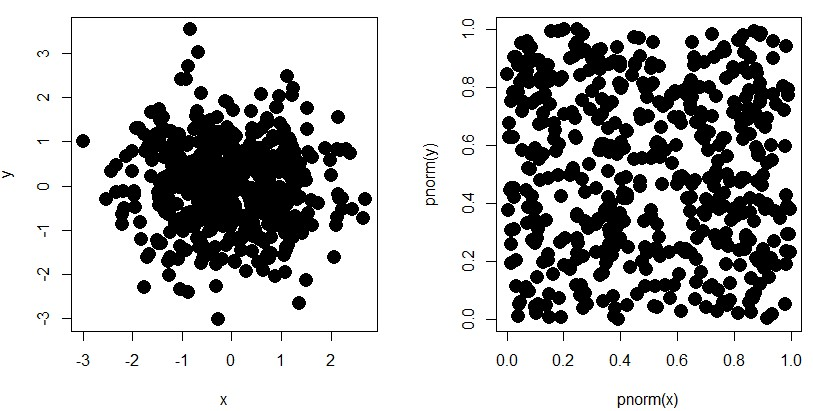
\includegraphics[width=0.75\linewidth]{ch-visualizer/figures/cdf}
		\caption[A plot of $y$ against $x$ after the CDF is applied in both
		directions.]{A plot of $y$ against $x$ with no transformation (left) 
		and after
			the CDF is applied in both directions (right). The code for this 
			example may be
			found in ~\ref{sec:appendicies:cdf}}
		\label{fig:visualizer:cdf}
	\end{center}
\end{figure}

Restricting the plot to a unit box allows analyst's visual systems to focus on
locations where there is low spatial frequency, which is ideal for detecting
dependence~\cite{hofert2016}. The effects of this can be progressively observed
by looking from the left to the right in
Figure~\ref{fig:visualizer:hofertoldford} below.

\begin{figure}[htb]
	\begin{center}
		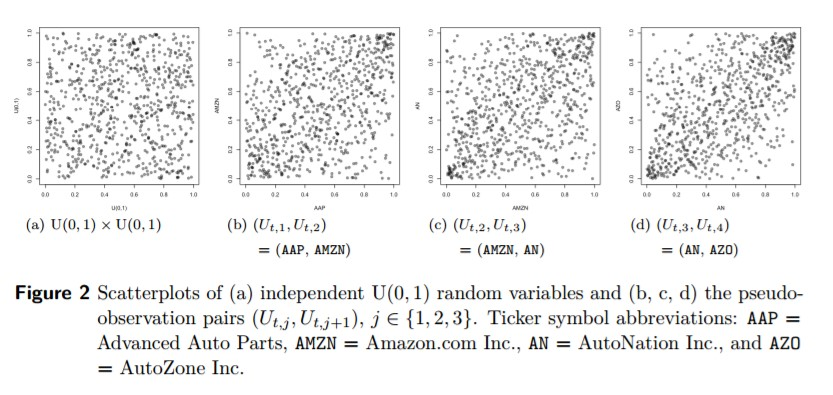
\includegraphics[width=0.75\linewidth]{ch-visualizer/figures/hofertoldford}
		\caption[Scatterplots of independent $U(0,1)$ random variables and the
		pseudo-observation pairs $(U_{t,j},U_{t,j+1}),j\in 
		\{1,2,3\}$.]{Scatterplots of
			(a) independent $U(0,1)$ random variables and (b,c,d) the 
			pseudo-observation
			pairs $(U_{t,j},U_{t,j+1}),j\in \{1,2,3\}$. Ticker abbreviations: 
			AAP = Advanced
			Auto Parts, AMZN = Amazon.com Inc, AN = AutoNation Inc., AZO = 
			AutoZone Inc.
			Images from Hofert and Oldford 2016~\cite{hofert2016}}
		\label{fig:visualizer:hofertoldford}
	\end{center}
\end{figure}

\subsection{Feature extraction from plot}
\label{sec:visualizer:features}

\subsubsection{Numerical features}

((Our goal is to quantify various features of a scatter plot. One category of
features are numerical features. These include Pearson correlation, tests of
independence, mutual information criterion, etc))

\subsubsection{Visual features}

((The other category of feature are visual. How many points are near the center
of the plot? How many points lie above the linear regression line? ))


